\documentclass{homework}
\usepackage[utf8]{inputenc}
\usepackage{enumerate}
\usepackage{graphicx}

\course{Ideals, Varieties, and Algorithms}
\title{Week 1}
\author{Andrew Li}

\begin{document}
    \maketitle

    \setcounter{section}{1}
    \setcounter{subsection}{2}
    \subsection{Problem 5}
    
    \begin{enumerate}[(a)]
        \item Show that the point $(x, y) = (\cosh(t), \sinh(t))$ always lies on $x^2 - y^2 = 1$. What portion of the hyperbola is covered?
        \item Show that a straight line meets a hyperbola in 0, 1, or 2 points, and illustrate your answer with a picture.
        \item Adapt the argument given at the end of the section to derive a parametrization of the hyperbola.
        \item The parametrization you found in part (c) is undefined for two values of $t$. Explain how this relates to the asymptotes of the hyperbola.
    \end{enumerate}
    
    \subsubsection*{Solution}
    \begin{enumerate}[(a)]
        \item By definition,
        \[\cosh(t) = \frac{e^t + e^{-t}}{2}, \quad\quad\quad \sinh(t) = \frac{e^t - e^{-t}}{2}\]
        Thus
        \begin{align*}
            \left(\frac{e^t + e^{-t}}{2}\right)^2 - \left(\frac{e^t - e^{-t}}{2}\right)^2 &= \frac{e^{2t} + 2 + e^{-2t} - e^{2t} + 2 - e^{-2t}}{4} \\
            &= 1.
        \end{align*}
        So the point $(\cosh(t), \sinh(t))$ lies on $x^2 - y^2 = 1$ for all $t$. This covers the right half of the hyperbola.
        
        \item We consider the cases where we have straight lines $x = a$ and $y = mx + b$ separately. When $x = a$, we have three cases
        \begin{figure*}[ht!]
            \fbox{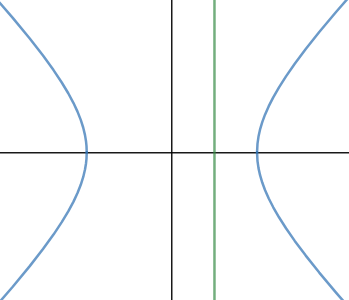
\includegraphics[width=.3\textwidth]{week1images/constant0.png}}\hfill
            \fbox{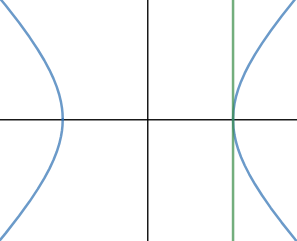
\includegraphics[width=.3\textwidth]{week1images/constant1.png}}\hfill
            \fbox{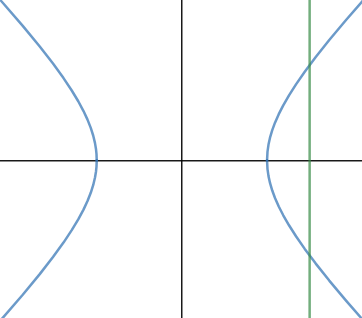
\includegraphics[width=.3\textwidth]{week1images/constant2.png}}
        \end{figure*} \\
        In particular, there can be no more than two solutions. If there are two, there is clearly one $(a, y)$ that lies on the hyperbola. Then, the only other solution is $(a, -y)$ since at most only two reals $y, -y$ can square to the same real $y^2$ (Fundamental Theorem of Algebra).
        
        Now when $y = mx+b$, we can employ a geometric argument. A line can intersect another line at most once in Euclidean plane. So, our line $y = mx+b$ can intersect each asymptote at most once. Since the hyperbola is bounded by these asymptotes, this means our line intersects the hyperbola in at most two places.
        \begin{figure}[h!]
            \centering
            \fbox{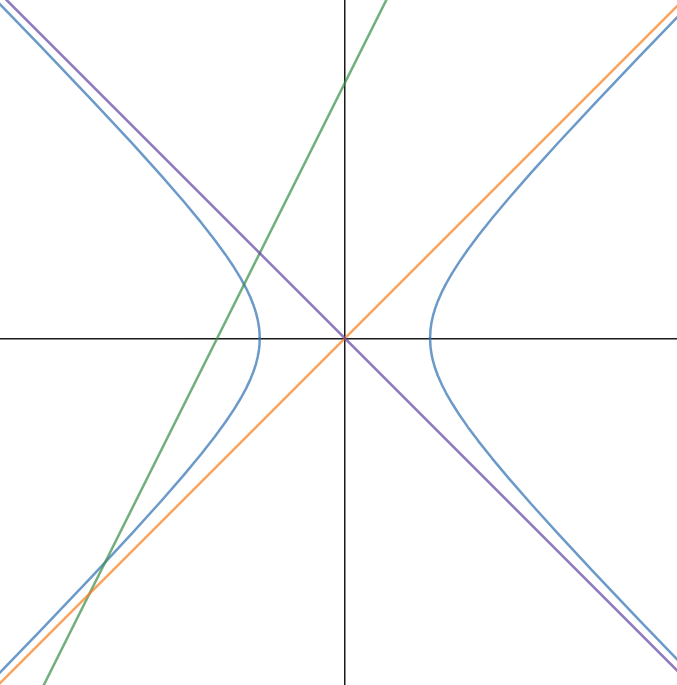
\includegraphics[scale=0.3]{week1images/lineh.png}}
            \caption{Hyperbola and general line}
        \end{figure}
        
        \item We can form a line from $(-1, 0)$ onto the hyperbola parametrized by slope $t \in \mathbb R$.
        \begin{figure}[h!]
            \centering
            \fbox{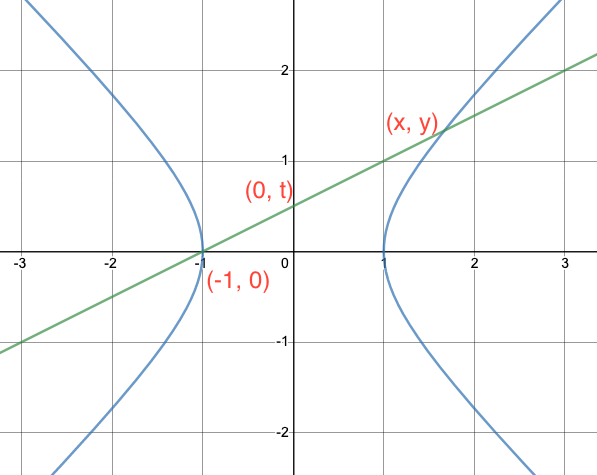
\includegraphics[scale=0.5]{week1images/hparam.png}}
            \caption{Parametrizing hyperbola with line of rational slope $t$}
        \end{figure}
        So we have the two equations
        \begin{align*}
            x^2 - y^2 &= 1 \\
            y &= t(x+1).
        \end{align*}
        Substituting, we have $x^2 - (t(x+1))^2 = 1$, which produces the quadratic
        \[(1-t^2)x^2 - 2t^2x - (1 - t^2) = 0.\]
        Since $(-1, 0)$ is a solution to both, we know $x+1$ is a factor of this quadratic. Factoring, we have
        \[(x+1)((1-t^2)x - (1+t^2)) = 0.\]
        The general parametrization is given when $(1-t^2)x - (1-t^2) = 0$, which yields
        \[x = \frac{1+t^2}{1-t^2}, \quad\quad\quad y = \frac{2t}{1-t^2}.\]
        
        \item This parametrization is undefined for $t = 1, -1$, which are exactly the slopes of the asymptotes. In particular, when $t = 1$, the line $y = t(x+1)$ crosses the hyperbola at $(-1, 0)$ by construction, but only there since $t = 1$ is the slope of one asymptote. Thus there is no $(x, y)$ like that pictured. A similar reason follows for $t = -1$ with the other asymptote.
    \end{enumerate}
    
\end{document}
